\documentclass[a4paper,10pt]{article}
\usepackage{trymtex}
\usepackage[backend=biber,style=alphabetic]{biblatex}
\usepackage{wrapfig}
\usetikzlibrary{arrows.meta,calc,positioning}
\addbibresource{bib/references.bib}

\begin{document}
\begin{titlepage}
    \newcommand{\HRule}{\rule{\linewidth}{0.5mm}}
    \begin{tikzpicture}[remember picture, overlay]
      % NTNU logo
      \node[anchor=north west, xshift=1.0cm, yshift=-1.0cm] at (current page.north west) {
        
\includegraphics[width=2.0cm]{figures/ntnu_logo_liten.png}
      };
    \end{tikzpicture}
  
    \center

    % Course code & title
    {\color{ntnu-blue}\sffamily\large TMA4212 \par}
    {\sffamily\Large Numerical Solution of Differential Equations by Difference Methods \par}
    
    \HRule
    \vspace{1.5cm}
  
    % Assignment title
    {\large\sffamily\bfseries Project 2\par}
    \vspace{0.3cm}
    {\Large\sffamily\textit{Solving the Poisson equation, and an Optimal Control Problem\\ using the Finite Element Method}\par}
  
    \vspace{0.5cm}
    \HRule
  
    \vfill
  
    % Author info
    \begin{minipage}{0.6\textwidth}
      \begin{flushleft}
        \large
        \textbf{Authors:}\\
        Haugen, Tor Ludvig Løvold \\
        Sæther, Trym\\ 
      \end{flushleft}
    \end{minipage}%
    \begin{minipage}{0.4\textwidth}
      \begin{flushright}
        \large
        \textbf{Semester:}\\
        Spring 2025
      \end{flushright}
    \end{minipage}
  
    % University logo/name
    \begin{center}
      {\color{ntnu-blue}\sffamily\Large Norwegian University of Science and Technology}\\
      \vspace{0.3cm}
      {\sffamily\large Department of Mathematical Sciences}
  
      \vspace{0.5cm}
      {\large\today}
    \end{center}
  
    \vspace{1cm}
  \end{titlepage}
  
  
  
\clearpage

\section{Introduction and Problem Statement}
We consider the one-dimensional Poisson equation
\[
	-u''(x) = f(x), \quad x \in \Omega=(0,1),
\]
with the (homogeneous) Dirichlet boundary conditions \(u(0)=u(1)=0\).
Our goal is to derive the (discrete) finite element method (FEM) using piecewise quadratic (\(\mathbb{P}_2\)) polynomials on a partition of the interval, implement the solver, and then confirm numerically the theoretical convergence rates of order \(\mathcal{O}(h^3)\) in the \(L^2\)-norm and \(\mathcal{O}(h^2)\) in the \(H^1\)-norm.

\subsection{Mesh and Basis Functions}
For quadratic finite elements, we partition $[0,1]$ into $M$ elements with $2M$ nodes, where each element has 3 nodes (2 endpoints and 1 midpoint).
The full node sequence is $0 = x_0 < x_2 < \cdots < x_{2M} = 1$, with elements $K_k = [x_{2k},x_{2k+2}]$ and widths $h_k = x_{2k+2} - x_{2k}$.
On this mesh, we define $V_h$ as the space of continuous piecewise quadratic functions.

\paragraph{Degrees of Freedom} With 3 nodes per element and accounting for shared nodes, a mesh with $M$ elements yields $2M+1$ total nodes. After imposing Dirichlet conditions, we have $\dim V_h = 2M-1$ degrees of freedom.

\subsection{Local Shape Functions}
On the reference element $\widehat{K}=[0,1]$, we choose the convenient reference nodes \(\xi_\beta=\{0,0.5,1\}\), where we define the local Lagrange basis functions
\[
	\Psi_{\alpha}(\xi_{\beta})
	= \delta_{\alpha\beta} =
	\begin{cases}
		\Psi_0(\xi) = 2\xi^2-3\xi+1 \\
		\Psi_1(\xi) = -4\xi^2+4\xi  \\
		\Psi_2(\xi) = 2\xi^2-\xi
	\end{cases} (\alpha,\beta=0,1,2).
\]
These functions are chosen such that they vanish at two of the three reference nodes and equal $1$ at the remaining node.

To map from the reference element $\widehat{K}$ to a physical element $K_k=[x_k,x_{k+1}]$, we use the affine transformation
\[
	\Phi_{K_k}:\,\widehat{K}\to K_k,\quad x=\Phi_{K_k}(\xi)=x_k+\xi\,h_k.
\]
Thus, the physical shape functions on $K_k$ are given by
\[
	\phi_{\alpha}^{K_k}(x) \;=\; \Psi_{\alpha}\!\Bigl(\frac{x-x_k}{h_k}\Bigr),\quad \alpha=0,1,2.
\]
Each $\phi_{\alpha}^{K_k}(x)$ is supported only on $K_k$.


\begin{wrapfigure}{r}{0.5\textwidth}
	\centering
	\begin{tikzpicture}[scale=2]
		% Reference element plot
		\begin{scope}[xshift=-1.0cm]
			% Grid
			\draw[very thin,color=gray!30] (-0.2,-0.2) grid[step=0.2] (1,1);
			\draw[->,thick] (-0.2,0) -- (1.2,0) node[right] {\(\xi\)};
			\draw[->,thick] (0,-0.2) -- (0,1.1) node[above] {\(\Psi(\xi)\)};

			% Reference points
			\fill (0,1) circle (0.5pt) node[left] {1};

			% Shape functions
			\draw[thick,blue,domain=0:1,samples=100] plot (\x,{2*\x*\x - 3*\x + 1})
			node[below] {\(\Psi_0(\xi)\)};
			\draw[thick,red,domain=0:1,samples=100] plot (\x,{-4*\x*\x + 4*\x})
			node[above left] {\(\Psi_1(\xi)\)};
			\draw[thick,green!50!black,domain=0:1,samples=100] plot (\x,{2*\x*\x - \x})
			node[left] {\(\Psi_2(\xi)\)};
		\end{scope}
		% Physical element plot
		\begin{scope}[xshift=1.0cm]
			% Grid
			\draw[very thin,color=gray!30] (-0.2,-0.2) grid[step=0.2] (1,1);
			\draw[->,thick] (-0.2,0) -- (1.2,0) node[right] {\(x\)};
			\draw[->,thick] (0,-0.2) -- (0,1.1) node[above] {\(\varphi_{k,\alpha}(x)\)};

			% Reference points
			\fill (0,1) circle (0.5pt) node[left] {1};

			% Shape functions
			\draw[thick,blue,domain=0:1,samples=100] plot (\x,{2*\x*\x - 3*\x + 1})
			node[below] {\(\varphi_{k,0}(x)\)};
			\draw[thick,red,domain=0:1,samples=100] plot (\x,{-4*\x*\x + 4*\x})
			node[above left] {\(\varphi_{k,1}(x)\)};
			\draw[thick,green!50!black,domain=0:1,samples=100] plot (\x,{2*\x*\x - \x})
			node[left] {\(\varphi_{k,2}(x)\)};
			% Element nodes
			\fill (0,0) circle (0.5pt) node[below] {\(x_{2k}\)};
			\fill (0.5,0) circle (0.5pt) node[below] {\(x_{2k+1}\)};
			\fill (1,0) circle (0.5pt) node[below] {\(x_{2k+2}\)};
		\end{scope}

		% Transformation arrow
		\node[above] at (0.5,0.25) {\(\overset{\Phi_{K_k}}{\Longrightarrow}\)};

	\end{tikzpicture}
	\caption{Reference functions $\Psi_\alpha(\xi)$ (left) and mapped physical functions $\varphi_{k,\alpha}(x)$ (right) under $\Phi_{K_k}$.}
	\label{fig:quadratic-shape-functions}
\end{wrapfigure}

\subsection{Global Shape Functions}
To form the global finite element space, we identify the degrees of freedom at the shared nodes between adjacent elements.
The resulting global basis functions satisfy the property
\[
	\varphi_j(x_\ell) \;=\; \delta_{j\ell},
\]
where the index $j$ runs over the total set of node and midpoint positions (excluding the two boundary nodes after imposing $v(0)=v(1)=0$). Thus, the final dimension of $V_h$ is $2N-1$.

Using this basis, any \(u_h \in V_h\) can be written as
\[
	u_h(x) = \sum_{j=1}^{2N-1} u_j\,\varphi_j(x)\,,
\]
where \(u_j\) are the unknown coefficients (corresponding to the values of \(u_h\) at each interior node or midpoint).
Substituting this expansion into the weak equation~\eqref{eq:weak_form} and choosing \(v_h=\varphi_i\) in turn yields a linear system \(A \mathbf{u} = \mathbf{b}\), as derived next.

\subsection{Variational Formulation}
We use the weak form of the Poisson problem: find $u \in \mathcal{H}^1_0(0,1)$ such that
\[
	a(u,v) = F(v), \quad \forall v \in \mathcal{H}^1_0(0,1),
\]
where $a(u,v) = \int_0^1 u'v'\,dx$ and $F(v) = \int_0^1 fv\,dx$. By the Galerkin method, we seek $u_h \in V_h$ such that $a(u_h,v_h) = F(v_h)$ for all $v_h \in V_h$. 
The Lax-Milgram theorem ensures a unique solution.
Expanding $u_h = \sum_j u_j\varphi_j$ and testing with each basis function $\varphi_i$ yields the linear system $A\mathbf{u} = \mathbf{b}$, where:
\[
	A_{ij} = \int_{0}^{1} \varphi_i'(x)\varphi_j'(x)\,dx, \quad 
	b_i = \int_{0}^{1} f(x)\varphi_i(x)\,dx.
\]

We compute these integrals element-by-element. For each element $K_k$, we calculate the local stiffness matrix and load vector:
\[
	A^{K_k}_{\alpha\beta} = \int_{K_k} (\phi_{\beta}^{K_k})' (\phi_{\alpha}^{K_k})'\,dx, \quad
	\mathbf{b}^{K_k}_\alpha = \int_{K_k} f(x)\phi_{\alpha}^{K_k}(x)\,dx,
\]
and then assemble them into the global system using appropriate local-to-global mappings.

\subsection{Assembly and Global System}
\begin{wrapfigure}{r}{0.4\textwidth}
	\centering
	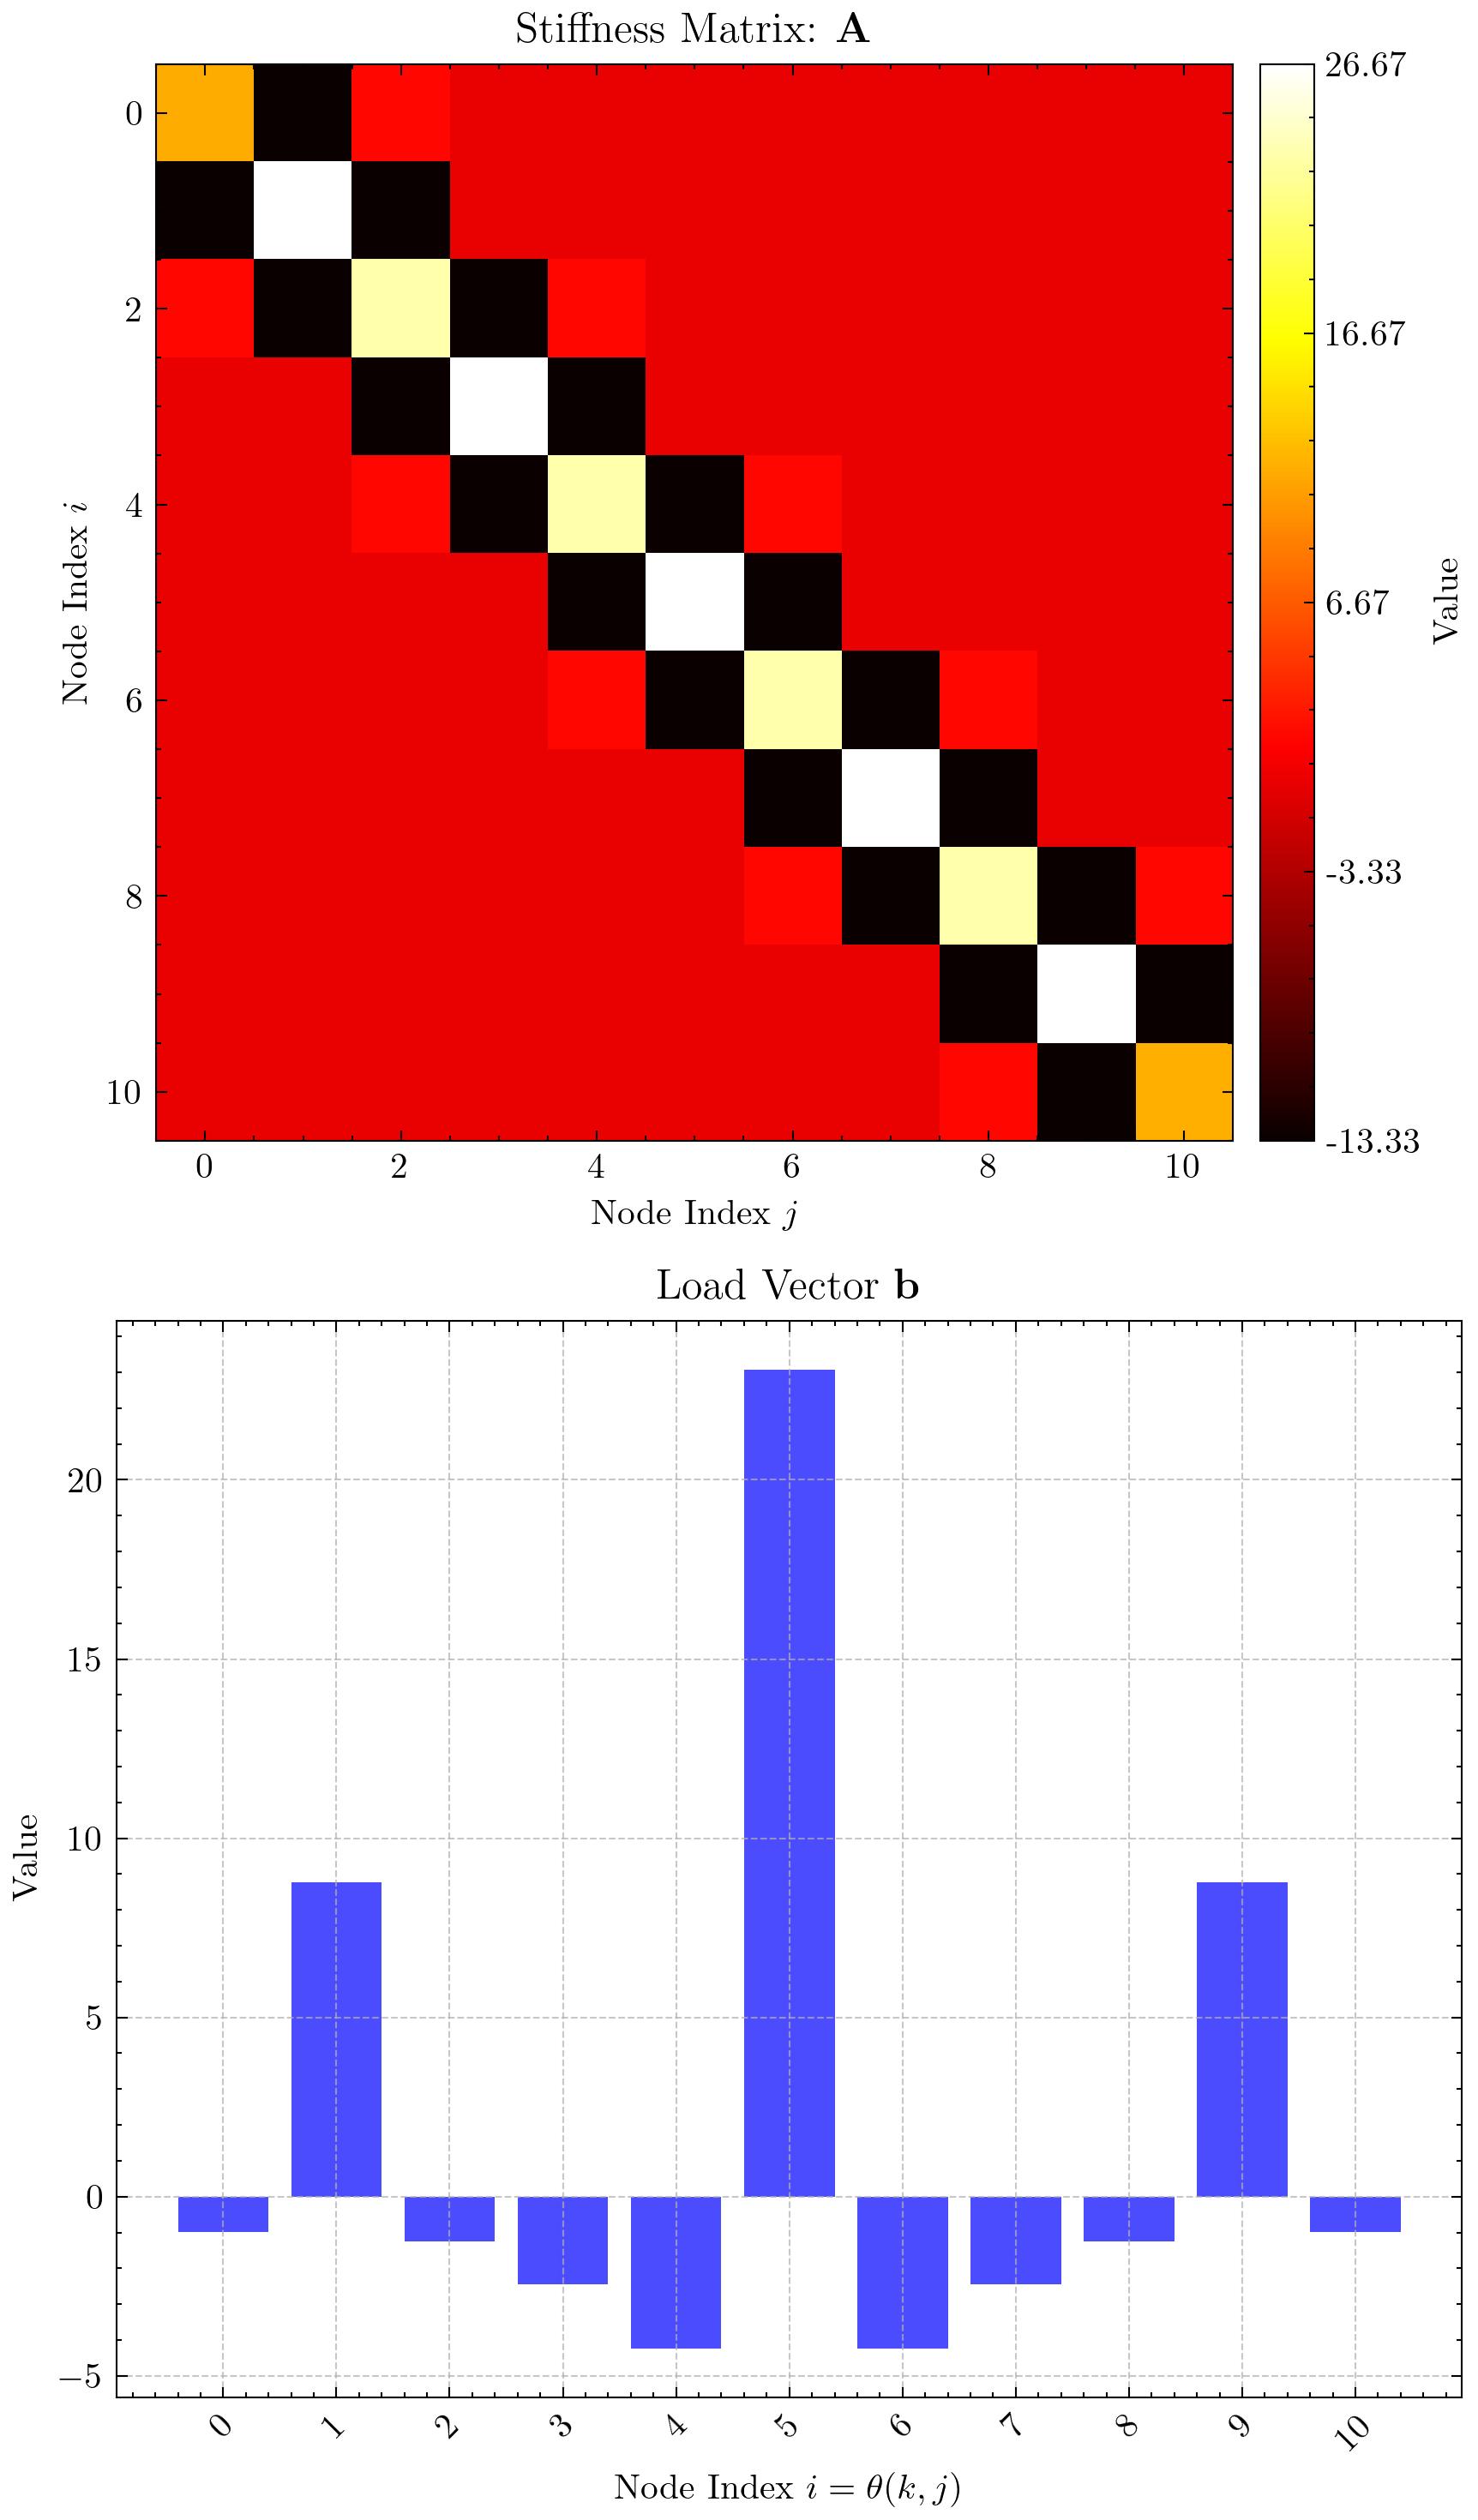
\includegraphics[width=0.3\textwidth]{figures/stiffness_matrix_complex.png}
	\caption{Global stiffness matrix \(A\) and load vector \(\mathbf{b}\) given in \ref{ex:simple} for \(M=5\) elements.}
	\label{fig:stiffness_load}
\end{wrapfigure}
Once the local matrices \(A^{K_k}\) and vectors \(\symbf{b}^{K_k}\) are computed for each element, they are assembled into the global matrix \(A\) and vector \(\mathbf{b}\) by summing the contributions from each element.
The assembly process uses a local-to-global mapping \(\theta(i,\alpha)=p\) to identify which global basis function \(\varphi_p\) corresponds to each local basis function \(\phi_\alpha^{K_k}\), ensuring that element contributions \(A^{K_k}_{\alpha\beta}, \symbf{b}^{K_k}_\alpha\) are properly summed into the appropriate entries of the global stiffness matrix  \(A_p\) and load vector \(\mathbf{b}_p\).

Note that if a node lies on the boundary (e.g., \(x_0\) or \(x_N\)), its corresponding basis function is not included in the global unknowns since the homogeneous Dirichlet condition \(u_h(0)=u_h(1)=0\) is enforced directly.
Consequently, the resulting global system is of size \((2N-1) \times (2N-1)\).

After assembly, we obtain the \emph{symmetric positive-definite} linear system.
\[
	A\,\mathbf{u} = \mathbf{b}.
\]

\subsection{Implementation}
We implemented our finite element solver in Python.
The code constructs the mesh and basis mappings, computes element matrices and vectors (using Simpson's rule),
assembles the global system, and solves it with a dense linear solver for simplicity.

\begin{algorithm}[H]
	\caption{Finite Element Assembly for $\mathbb{P}_2$ Elements}
	\label{alg:FEM_assembly}
	\SetKwInOut{Input}{Input}
	\SetKwInOut{Output}{Output}
	\Input{\(f\), \(M\), mesh data with global node mapping}
	Initialize \(A \in \mathbb{R}^{(2M-1) \times (2M-1)}\) and \(b \in \mathbb{R}^{2M-1}\) to zero\;
	\For{each element \(k = 0,1,\ldots,M-1\)}{
		\(h_k \leftarrow x_{2k+2} - x_{2k}\)\;
		Compute \texttt{A\_loc} = localStiffnessMatrix\((h_k)\) and \texttt{b\_loc} = localLoadVector\((h_k, f)\)\;
		\For{local indices \((\alpha,\beta) \in \{0,1,2\} \times \{0,1,2\}\)}{
			Map to global indices: \(I = \text{global\_index}[k][\alpha]\), \(J = \text{global\_index}[k][\beta]\)\;
			\(A[I,J] \mathrel{+}= \texttt{A\_loc}[\alpha,\beta]\)\;
			\If{\(\beta = 0\)}{
				\(b[I] \mathrel{+}= \texttt{b\_loc}[\alpha]\)\;
			}
		}
	}
	\Output{Global system matrix \(A\) and load vector \(b\)}
\end{algorithm}
\subsection{Numerical Experiments and Results}
We tested the solver on two example problems with known exact solutions.
\begin{example}{Simple Poisson Problem}{simple}
	We first consider the simple Poisson problem \(-u''(x) = 1\) with \(x \in [0,1]\) and \(u(0)=u(1)=0\), whose exact solution is \(u(x) = \tfrac12\,x(1-x)\).
\end{example}
\begin{figure}[H]
	\centering
	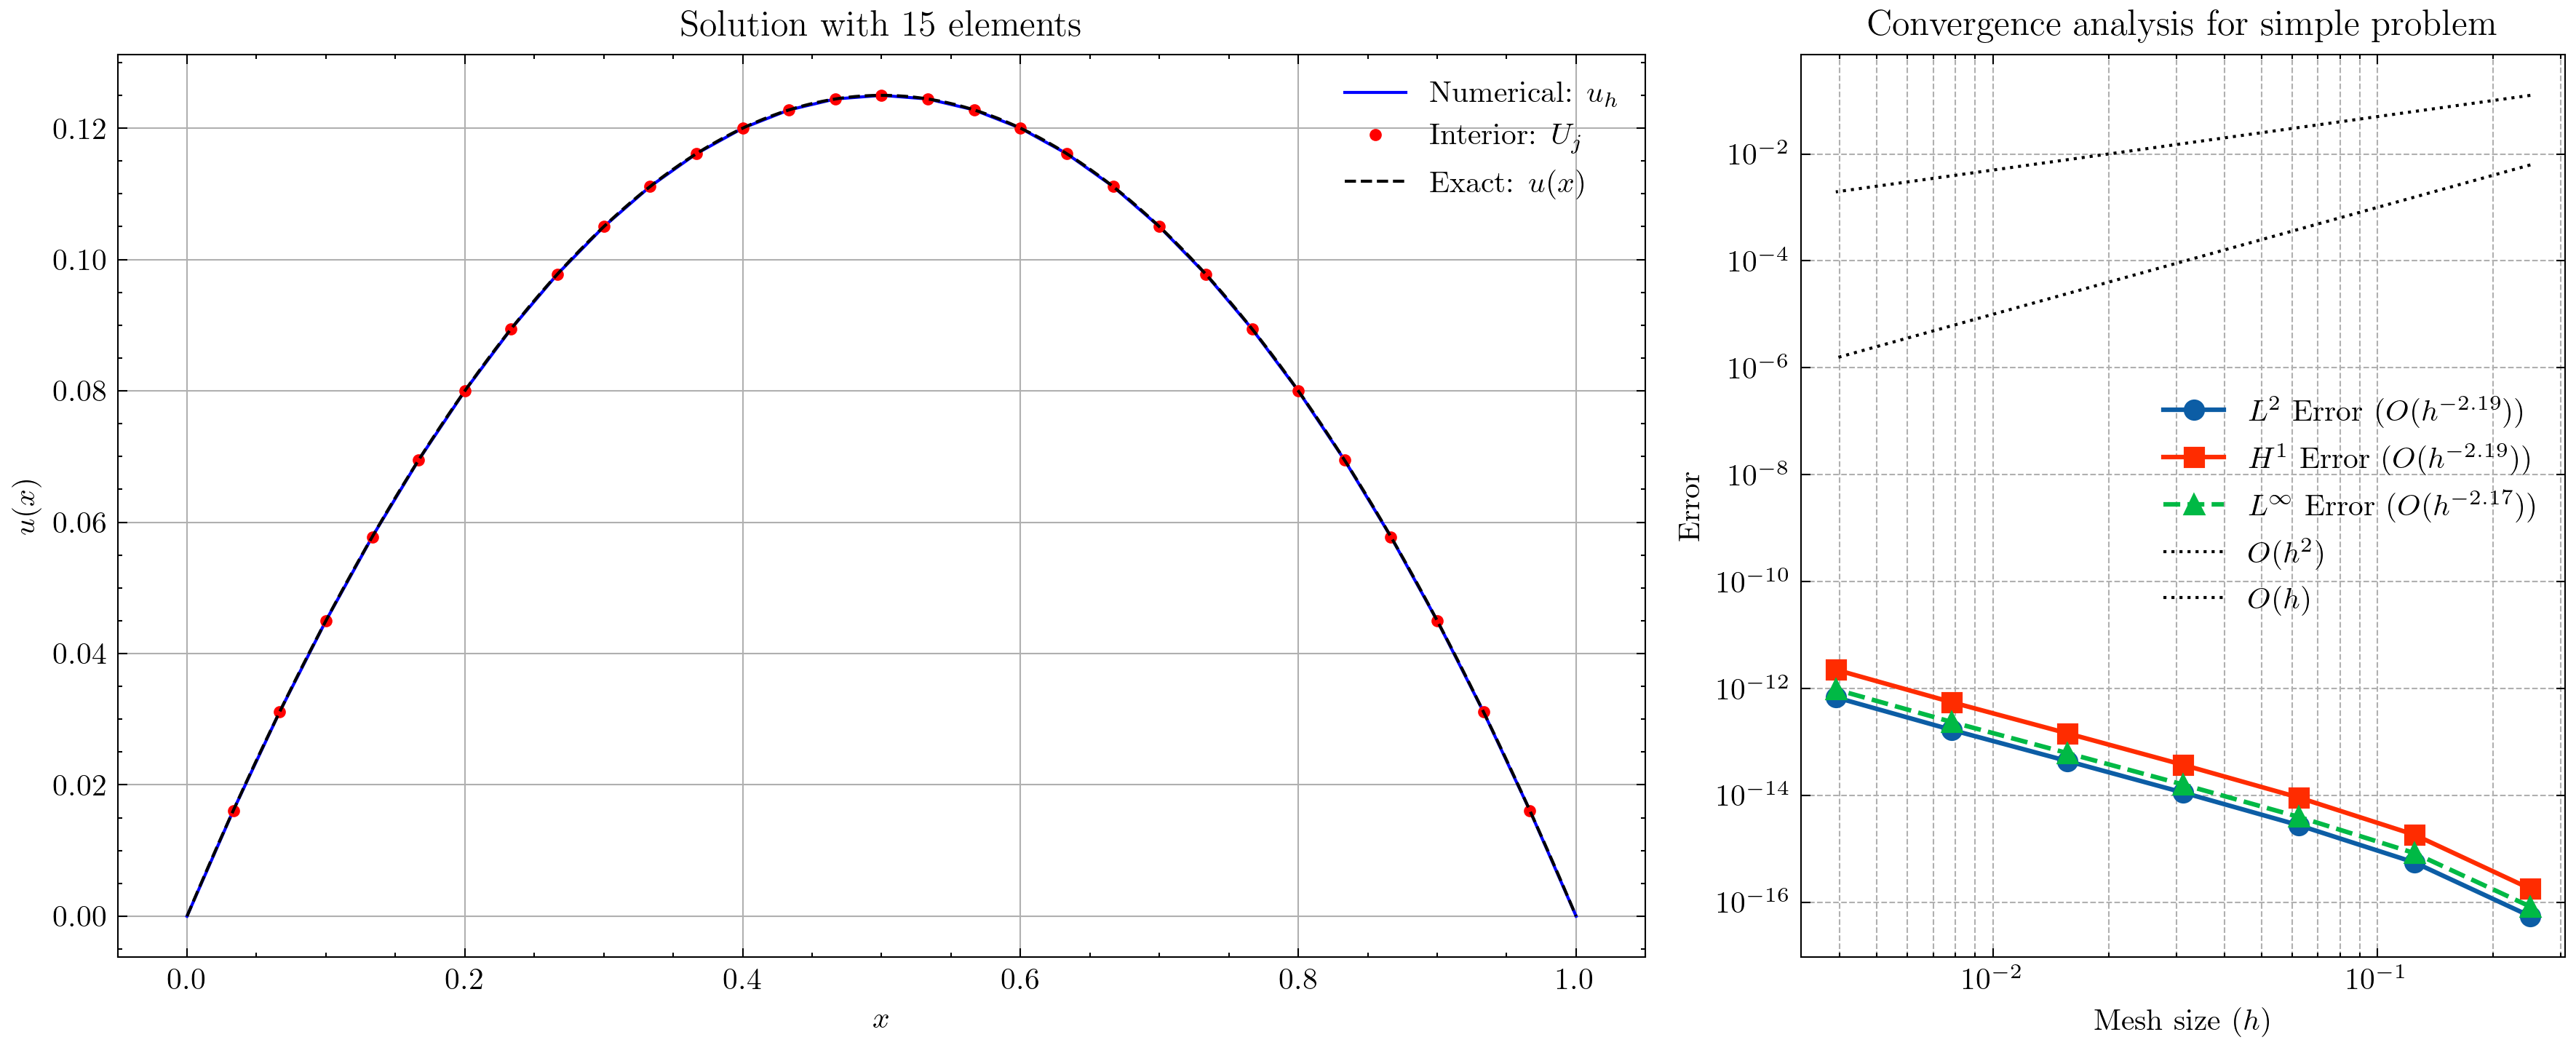
\includegraphics[width=0.99\textwidth]{figures/convergence_simple.png}
	\caption{FEM solution vs. exact solution (top), error convergence rates (bottom left), and error distribution (bottom right).}
	\label{fig:solution_simple}
\end{figure}
\begin{table}[H]
	\centering
	\begin{tabular}{|c|c|S[table-format=1.2e-2]|c|S[table-format=1.2e-2]|c|S[table-format=1.2e-2]|c|}
		\hline
		\rowcolor{blue!15}
		\rowcolor{blue!15} \textbf{M} & \textbf{h} & {\textbf{$L^2$ Error}} & \textbf{Rate} & {\textbf{$L^\infty$ Error}} & \textbf{Rate} & {\textbf{$H^1$ Error}} & \textbf{Rate} \\
		\hline
		10                            & 1.00e-01   & 3.19e-16               & --            & 5.00e-16                    & --            & 1.01e-14               & --            \\
		\rowcolor{blue!5}
		20                            & 5.00e-02   & 1.21e-15               & -1.92         & 1.75e-15                    & -1.81         & 2.14e-14               & -1.09         \\
		40                            & 2.50e-02   & 5.50e-15               & -2.18         & 8.08e-15                    & -2.21         & 4.92e-14               & -1.20         \\
		\rowcolor{blue!5}
		80                            & 1.25e-02   & 2.61e-14               & -2.24         & 3.73e-14                    & -2.21         & 1.23e-13               & -1.32         \\
		\hline
	\end{tabular}
	\caption{Convergence analysis for \ref{fig:solution_simple}.}
	\label{tab:convergence_simple}
\end{table}

Since the exact solution is quadratic, our finite element method should be exact for any mesh with $M \geq 4$ elements,
However, when solving the linear system on increasingly refined (uniform) mesh, we observe errors on the order of machine epsilon.
\begin{remark}{Machine epsilon}{}
	The \emph{machine epsilon} is the smallest number that, when added to 1.0, results in a number different from 1.0 in floating-point arithmetic.
\end{remark}

In practice, the computed solution is exact up to roundoff error. The error tends to increase slightly for finer meshes because the larger linear systems require more floating-point operations:
\[
	\text{Number of operations} \propto \mathcal{O}(M^3)
\]

\begin{example}{Complex Poisson Problem}{complex}
	We also tested our solver on a more complex problem with a highly oscillatory source term:
	\[
		-u''(x) = e^{\sin(5\pi x)}\left[25\pi^2 x(1-x)(\sin(5\pi x) - \cos^2(5\pi x)) + 10\pi (2x-1)\cos(5\pi x) + 2\right]
	\]
	with the exact solution \(u(x) =\sqrt{\sin(x)} + 5e^{-100x}\cos(x).\)
\end{example}
\begin{figure}[H]
	\centering
	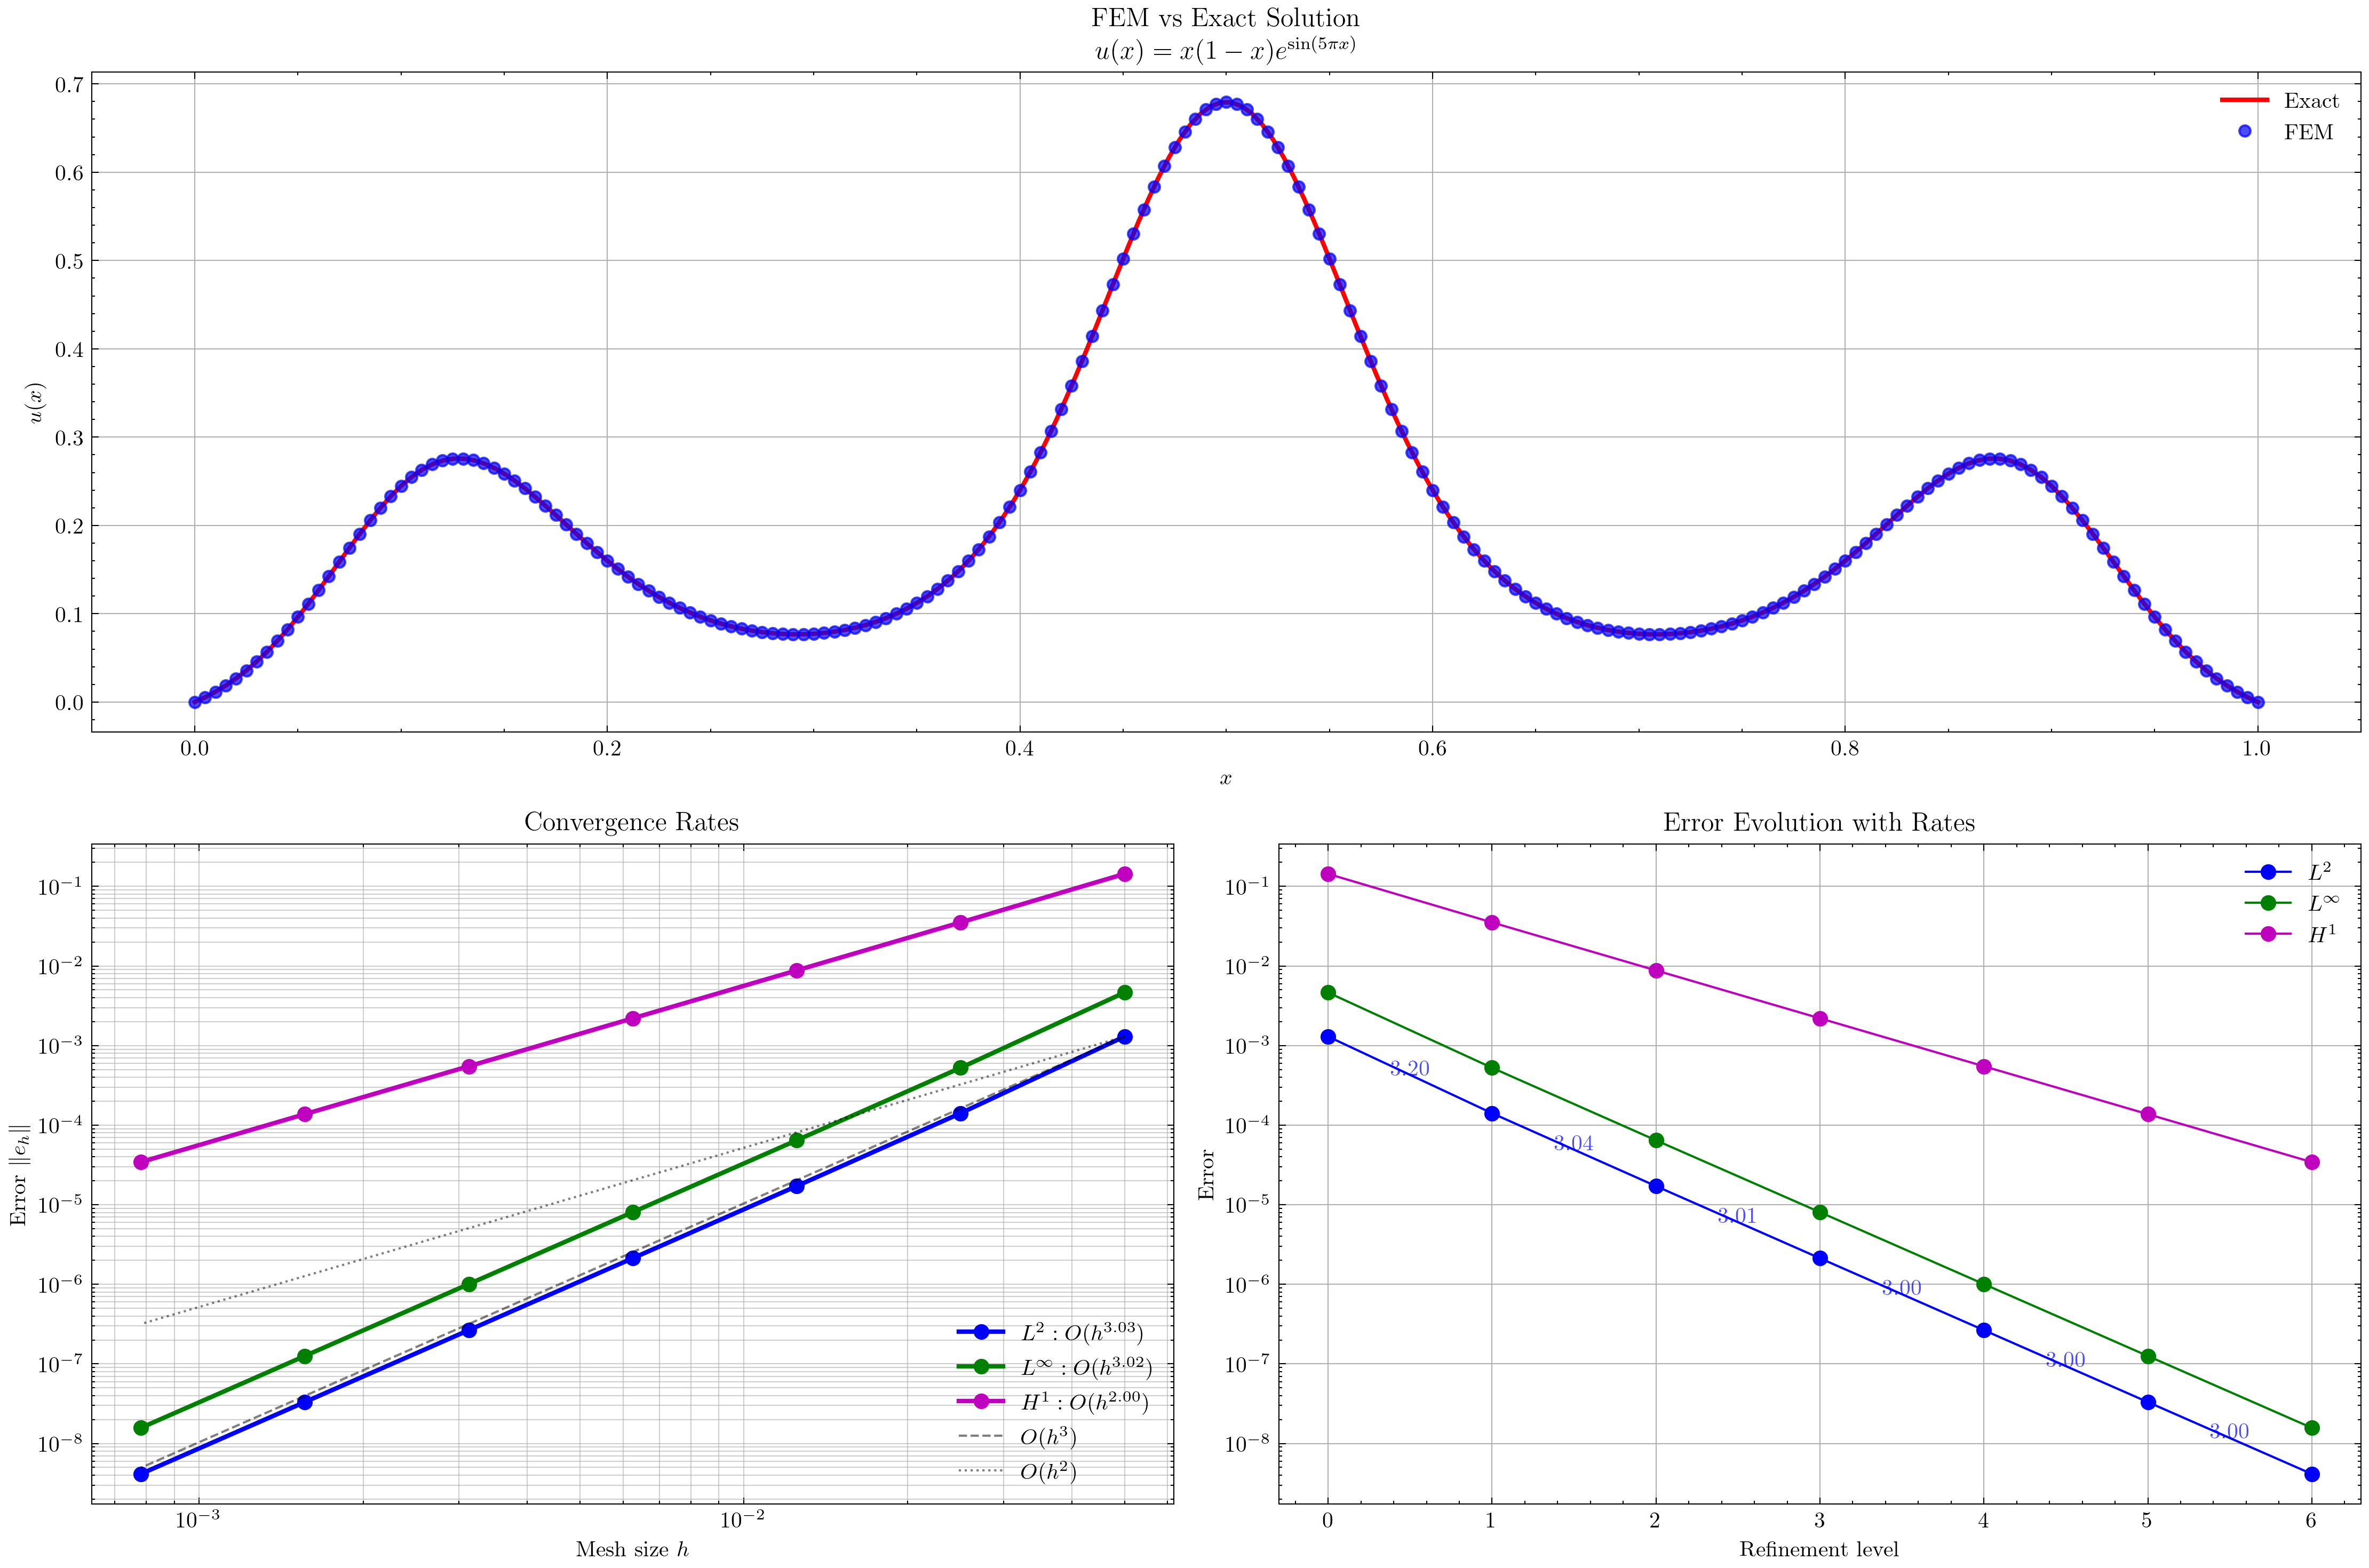
\includegraphics[width=0.95\textwidth]{figures/convergence_complex.png}
	\caption{Comparison of FEM solution \(u_h(x)\) with the exact solution \(u(x)\) and convergence rates for a complex example.}
	\label{fig:solution_complex}
\end{figure}
\begin{table}[H]
	\centering
	\begin{tabular}{|c|c|S[table-format=1.2e-2]|c|S[table-format=1.2e-2]|c|S[table-format=1.2e-2]|c|}
		\hline
		\rowcolor{blue!20} \textbf{M} & \textbf{h} & {\textbf{L² Error}} & \textbf{Rate} & {\textbf{L∞ Error}} & \textbf{Rate} & {\textbf{H¹ Error}} & \textbf{Rate} \\
		\hline
		10                            & 1.00e-01   & 1.19e-01            & --            & 2.38e-01            & --            & 7.88e-01            & --            \\
		\rowcolor{blue!5}
		20                            & 5.00e-02   & 1.30e-03            & 6.51          & 4.62e-03            & 5.69          & 1.42e-01            & 2.47          \\
		40                            & 2.50e-02   & 1.41e-04            & 3.20          & 5.25e-04            & 3.14          & 3.52e-02            & 2.02          \\
		\rowcolor{blue!5}
		80                            & 1.25e-02   & 1.71e-05            & 3.04          & 6.44e-05            & 3.03          & 8.80e-03            & 2.00          \\
		160                           & 6.25e-03   & 2.12e-06            & 3.01          & 8.05e-06            & 3.00          & 2.20e-03            & 2.00          \\
		\hline
	\end{tabular}
	\caption{Convergence analysis for \ref{fig:solution_complex}.}
	\label{tab:convergence_detailed}
\end{table}

\subsection{Theoretical Error Analysis and Convergence Rate}
Standard finite element theory establishes that for degree-$p$ elements, the error converges as $\mathcal{O}(h^p)$ in the $H^1$-norm and $\mathcal{O}(h^{p+1})$ in the $L^2$-norm, provided the exact solution has sufficient regularity ($u \in H^{p+1}(\Omega)$)\cite{brenner2008mathematical, quarteroni2009numerical}.
For our quadratic elements ($p=2$), we have:

\begin{theorem}{Optimal Convergence for $\mathbb{P}_2$ Elements}{theorem:p2convergence}
	Let $u \in H^3(\Omega)$ be the exact solution of the Poisson problem and $u_h \in V_h$ be the finite element solution using quadratic ($\mathbb{P}_2$) elements. Then there exists a constant $C > 0$ independent of the mesh size $h$ such that:
	\begin{align}
		\|u - u_h\|_{L^2(\Omega)} & \leq C h^3 \|u\|_{H^3(\Omega)}, \\
		\|u - u_h\|_{H^1(\Omega)} & \leq C h^2 \|u\|_{H^3(\Omega)}.
	\end{align}
\end{theorem}

\begin{proof}{}{}
	The proof consists of two main parts:
	\textit{Step 1: $H^1$-error estimate.}
	By interpolation theory, for any $u \in H^3(\Omega)$, the quadratic interpolant satisfies:
	\begin{align}
		\|u - I_h u\|_{H^1(\Omega)} & \leq C_1 h^2 \|u\|_{H^3(\Omega)}.
	\end{align}

	By Céa's lemma \cite{ciarlet1978finite}, the Galerkin solution $u_h$ is quasi-optimal in the $H^1$ norm:
	\begin{align}
		\|u - u_h\|_{H^1(\Omega)} & \leq C_2 \inf_{v_h \in V_h} \|u - v_h\|_{H^1(\Omega)} \\
		                          & \leq C_2 \|u - I_h u\|_{H^1(\Omega)}                  \\
		                          & \leq C_2 C_1 h^2 \|u\|_{H^3(\Omega)}.
	\end{align}

	\textit{Step 2: $L^2$-error estimate via Aubin-Nitsche duality.}
	Consider the auxiliary problem: find $\phi \in H^1_0(\Omega)$ such that $-\Delta \phi = u - u_h$ with $\phi = 0$ on $\partial\Omega$. Then:
	\[
		\|u - u_h\|^2_{L^2(\Omega)} = \int_\Omega (u - u_h)(-\Delta \phi) \, dx = \int_\Omega \nabla(u - u_h) \cdot \nabla(\phi - I_h\phi) \, dx
	\]
	where we used Galerkin orthogonality.
	Applying Cauchy-Schwarz and interpolation estimates:
	\[
		\|u - u_h\|^2_{L^2(\Omega)} \leq \|u - u_h\|_{H^1(\Omega)} \|\phi - I_h\phi\|_{H^1(\Omega)} \leq C_3 h \|u - u_h\|_{H^1(\Omega)} \|\phi\|_{H^2(\Omega)}
	\]
	Since $\|\phi\|_{H^2(\Omega)} \leq C_4 \|u - u_h\|_{L^2(\Omega)}$ by elliptic regularity, we get:
	\(
	\|u - u_h\|^2_{L^2(\Omega)} \leq C_5 h \|u - u_h\|_{H^1(\Omega)} \|u - u_h\|_{L^2(\Omega)}
	\)
	Dividing by $\|u - u_h\|_{L^2(\Omega)}$ and using the $H^1$ estimate from Step 1:
	\begin{align*}
		\|u - u_h\|_{L^2(\Omega)} & \leq C_5 h \|u - u_h\|_{H^1(\Omega)}             \\
		                          & \leq C_5 C_2 C_1 h \cdot h^2 \|u\|_{H^3(\Omega)} \\
		                          & = C h^3 \|u\|_{H^3(\Omega)}
	\end{align*}
	Which completes the proof.\qed
\end{proof}

Our numerical experiments in Tables \ref{tab:convergence_simple} and \ref{tab:convergence_detailed} confirm the theoretical convergence rates.
The observed rates match exactly the expected values: third-order ($\mathcal{O}(h^3)$) convergence in the $L^2$-norm and second-order ($\mathcal{O}(h^2)$) convergence in the $H^1$-norm, validating both our implementation and the theoretical analysis.

\section{Optimal Control Problem}
\label{sec:optimal_control}

\subsection{Problem Formulation}
We consider an optimal control problem for heating/cooling a physical domain \(\Omega=(0,1)\).
Given a target temperature profile \(y_d \in L^2(\Omega)\) and a control cost parameter \(\alpha > 0\), we seek to minimize
\[
	J(y,u) = \frac{1}{2}\int_0^1 |y-y_d|^2\,dx + \frac{\alpha}{2}\int_0^1 u^2\,dx,
\]
subject to \(y\) solving the Poisson equation with homogeneous Dirichlet conditions:
\[
	-\Delta y = u \quad\text{in }\Omega, \qquad y(0) = y(1) = 0.
\]
Here \(u\) represents the distributed heat source/sink (control) and \(y\) is the resulting temperature (state).
We discretize this optimal control problem using finite elements:
\[
	\min_{u_h,y_h\in V_h} \frac{1}{2}\|y_h - \bar{y}_d\|^2_{L^2(\Omega)} + \frac{\alpha}{2}\|u_h\|^2_{L^2(\Omega)}
\]
subject to
\[
	a(y_h,v) = \langle u_h,v \rangle_{L^2(\Omega)} \quad \forall v\in V_h,
\]
where \(\bar{y}_d\) is the interpolation of \(y_d\) onto \(X^2_h\), \(V_h = X^2_h \cap H^1_0(\Omega)\), and \(a\) is the bilinear form previously discussed.

\subsection{Discretization of the OCP}
First, we expand the objective function \(J\), state \(y(u)\), desired state \(y_d\) and control variable \(u\) in terms of the discrete basis functions:
\begin{align*}
	\bar{y}_d(x)                        & = \sum_{j=1}^{2N-1} (\bar{y}_d)_j \varphi_j(x), \quad
	y_h(x) = \sum_{j=1}^{2N-1} y_j \varphi_j(x), \quad
	u_h(x) = \sum_{j=1}^{2N-1} u_j \varphi_j(x)                                                             \\
	\|y_h - \bar{y}_d\|^2_{L^2(\Omega)} & =
	\int_0^1 \left(\sum_{j=1}^{2N-1} (y_j-(\bar{y}_d)_j)\varphi_j(x)\right)^2 dx =
	\sum_{i,j=1}^{2N-1} (y_i - (\bar{y}_d)_i)(y_j - (\bar{y}_d)_j) \int_0^1 \varphi_i(x) \varphi_j(x) \, dx \\
	\|u_h\|^2_{L^2(\Omega)}             & =
	\int_0^1 \left(\sum_{j=1}^{2N-1} u_j \varphi_j(x)\right)^2 dx =
	\sum_{i,j=1}^{2N-1} u_i u_j \int_0^1 \varphi_i(x)\varphi_j(x) \, dx
\end{align*}
This is equivalent to the \(L^2(\Omega)\) inner product of two polynomial approximations, which satisfies the identity:
\[
	\langle u, v \rangle_{L^2(\Omega)} = \sum_{i,j} u_i v_j \int_\Omega \varphi_i(x) \varphi_j(x) \, dx = \mathbf{u}^T M \mathbf{v}
\]
where \(M\) is the mass matrix, with elements \(M_{ij} = \int_\Omega \varphi_i(x) \varphi_j(x) \, dx\).
Thus, the objective function can be expressed as:
\[
	G(\mathbf{y},\mathbf{u}) = \frac{1}{2}(\mathbf{y}-\mathbf{\bar{y}_d})^T M (\mathbf{y}-\mathbf{\bar{y}_d}) + \frac{\alpha}{2} \mathbf{u}^T M \mathbf{u}
\]
For the constraint \(a(y_h,v) = \langle u_h,v \rangle_{L^2(\Omega)}\), testing with \(v = \varphi_i\) for \(i=1,\dots,2N-1\):
\[
	\sum_{j=1}^{2N-1} y_j a(\varphi_j,\varphi_i) = \sum_{j=1}^{2N-1} u_j \langle \varphi_j,\varphi_i \rangle_{L^2(\Omega)}
\]
By definition, the stiffness matrix \(K\) is given by \(K_{ij} = a(\varphi_j,\varphi_i)\) and the mass matrix \(M\) by \(M_{ij} = \langle \varphi_j,\varphi_i \rangle_{L^2(\Omega)}\), so the constraint becomes:
\[
	K \mathbf{y} = M \mathbf{u}
\]
Thus, \(B = A\), the stiffness matrix, and \(F = M\), the mass matrix.

\subsection{Lagrangian multipliers and critical points}
We discretize both $y(x)$ and $u(x)$ in the same $\mathbb{P}_2$ finite element space $V_h = X_h^2 \cap H_0^1(0,1)$, representing them as $y_h(x)=\sum_j y_j\varphi_j(x)$ and $u_h(x)=\sum_j u_j\varphi_j(x)$. This yields the matrix form of our objective function:
\[
	G(\mathbf{y},\mathbf{u}) = \frac{1}{2}(\mathbf{y}-\mathbf{\bar{y}_d})^T M(\mathbf{y}-\mathbf{\bar{y}_d}) + \frac{\alpha}{2}\,\mathbf{u}^T M\,\mathbf{u},
\]
where $M_{ij}=\int_\Omega \varphi_i(x)\varphi_j(x)\,dx$ is the mass matrix and $\mathbf{\bar{y}_d}$ contains the coefficients of interpolated $y_d$.

The PDE constraint in weak form becomes the linear system $Ky = Mu$, where $K_{ij}=\int_0^1 \varphi_i'\varphi_j'\,dx$ is the stiffness matrix.
We introduce Lagrange multipliers $\lambda$ to enforce the constraint, leading to the Lagrangian:
\[
	\mathcal{L}(y,u,\lambda) = G(y,u) - \lambda^T(Ky - Mu),
\]
where $\lambda$ is the vector of Lagrange multipliers corresponding to the constraint $Ky - Mu = 0$.

Finding the gradient of the Lagrangian with respect to $y$, $u$, and $\lambda$ gives the necessary optimality conditions (Karush-Kuhn-Tucker conditions):
\begin{align*}
	\nabla_y \mathcal{L}       & = M(y-y_d) - K\lambda = 0,  \\
	\nabla_u \mathcal{L}       & = \alpha Mu + M\lambda = 0, \\
	\nabla_\lambda \mathcal{L} & = Ky - Mu = 0.
\end{align*}
Rearranging these equations leads to the block--matrix system, that we can solve directly to obtain the optimal state $y_h$ and control $u_h$.
\[
	\begin{pmatrix}
		M & \alpha K \\
		K & -M
	\end{pmatrix}
	\begin{pmatrix}
		y \\
		u
	\end{pmatrix}
	=
	\begin{pmatrix}
		My_d \\
		0
	\end{pmatrix}, 
\]

\subsection{Numerical experiments}
\label{sec:numericalOCP}
To validate our optimal control approach, we conduct a series of numerical experiments that investigate how different target functions and control costs affect the solution behavior. We implement the finite element solver using quadratic elements on a uniform mesh with $M=100$ elements.

The OCP we consider is:
\[
	\min_{y,u} \; \tfrac12 \|y - y_d\|_{L^2(0,1)}^2 \;+\; \tfrac{\alpha}{2}\,\|u\|_{L^2(0,1)}^2
	\quad \text{subject to} \quad
	-y'' = u,\; y(0)=y(1)=0,
\]
where the parameter $\alpha$ represents the trade-off between state tracking accuracy and control cost. We examine three representative values: $\alpha \in \{10^{-2}, 10^{-4}, 10^{-6}\}$, ranging from relatively expensive control ($\alpha=10^{-2}$) to nearly unconstrained control ($\alpha=10^{-6}$).

We consider three cases for the target function $y_d$:
\begin{enumerate}
	\item \textbf{Case~1:} $y_d(x) = 0.5\,x\,(1-x)$, a smooth function in $H^1_0(0,1)$.
	\item \textbf{Case~2:} $y_d(x) = 1$, a constant function not vanishing at the boundaries (thus $y_d\notin H^1_0$).
	\item \textbf{Case~3:} $y_d(x)$ is the characteristic function of $[0.25,0.75]$, a discontinuous target (also not in $H^1_0$).
\end{enumerate}
These cases represent increasingly challenging targets, from a compatible smooth function to a discontinuous one, allowing us to observe how the method handles different levels of regularity.
\paragraph{Case 1 ($y_d \in H^1_0$):}
For large $\alpha = 10^{-2}$, the solution prefers minimal control ($u_h \approx 0$), so $y_h$ remains near the homogeneous solution $0$.

For $\alpha=10^{-4}$ decreases, $y_h$ closely matches $y_d$, with $u_h$ approaching the exact forcing needed to reproduce $y_d(x) = 0.5x(1-x)$.

For small $\alpha=10^{-6}$, we found $y_h \approx y_d$ and $u_h \approx 1$, since $-y_d''=1$.

\begin{figure}[htbp]
    \centering
    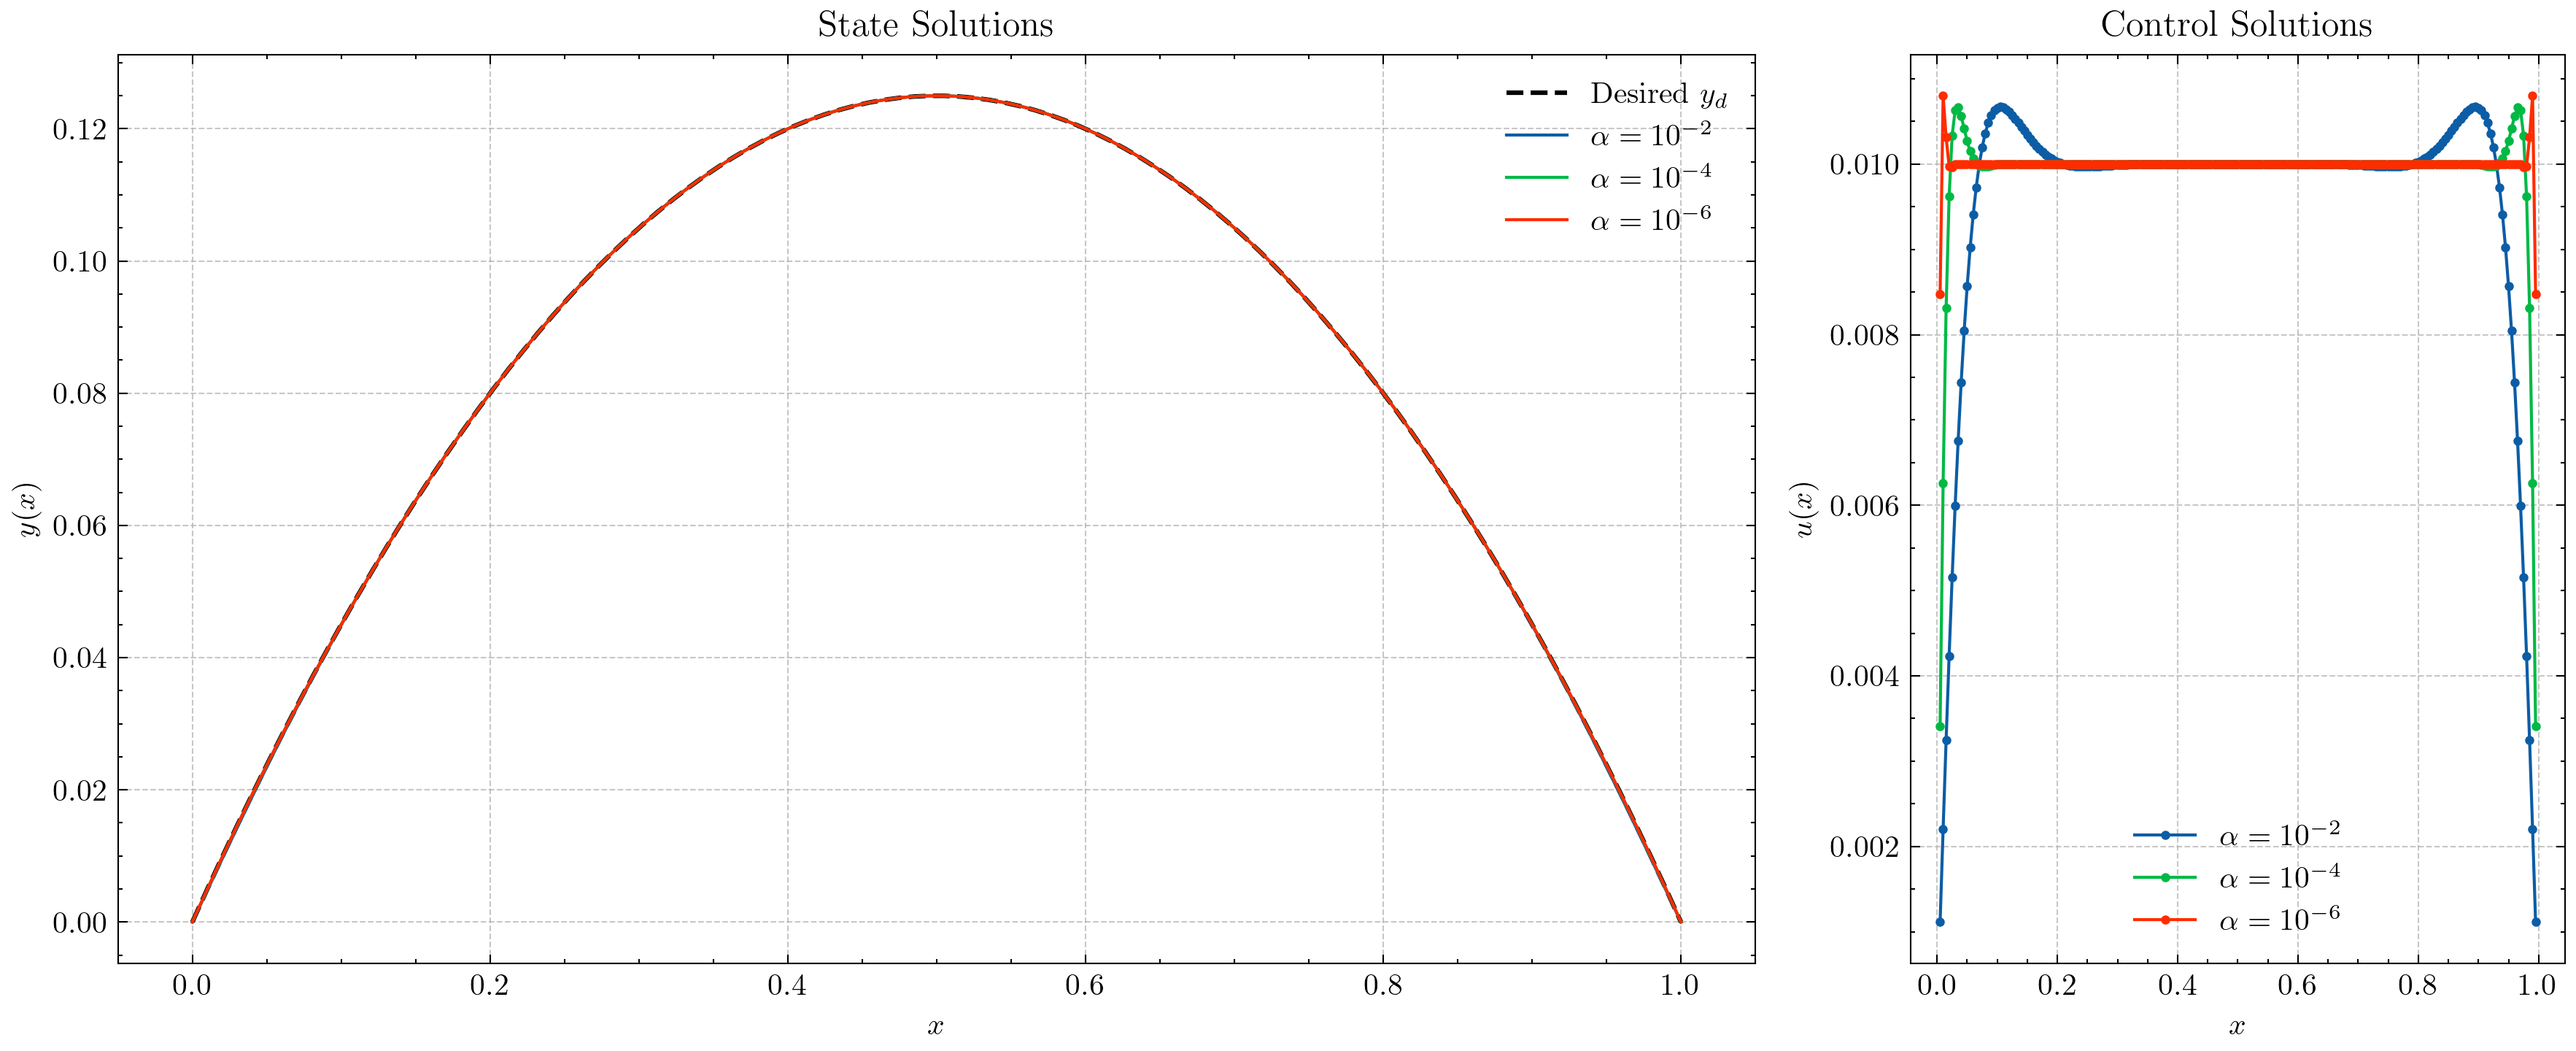
\includegraphics[width=0.95\textwidth]{figures/ocp_case1.png}
    \caption{Case~1 results: optimal state $y_h$ vs.\ target $y_d$ (left), and optimal control $u_h$ (right) for varying $\alpha$.}
    \label{fig:opt_control_case1_short}
\end{figure}

\paragraph{Case 2 (constant $y_d \notin H^1_0$):}
Since $y_d(x)=1$ cannot be met at $x=0,1$, $y_h$ stays near zero for large $\alpha$.

For smaller $\alpha$, the control exerts significant effort near the boundaries to \enquote{lift} $y_h$ toward $\approx1$ in the interior. 

In particular, at $\alpha=10^{-6}$, $y_h\approx1$ in much of $(0,1)$, with $u_h$ showing large spikes at $x=0$ and $x=1$.

\begin{figure}[htbp]
    \centering
    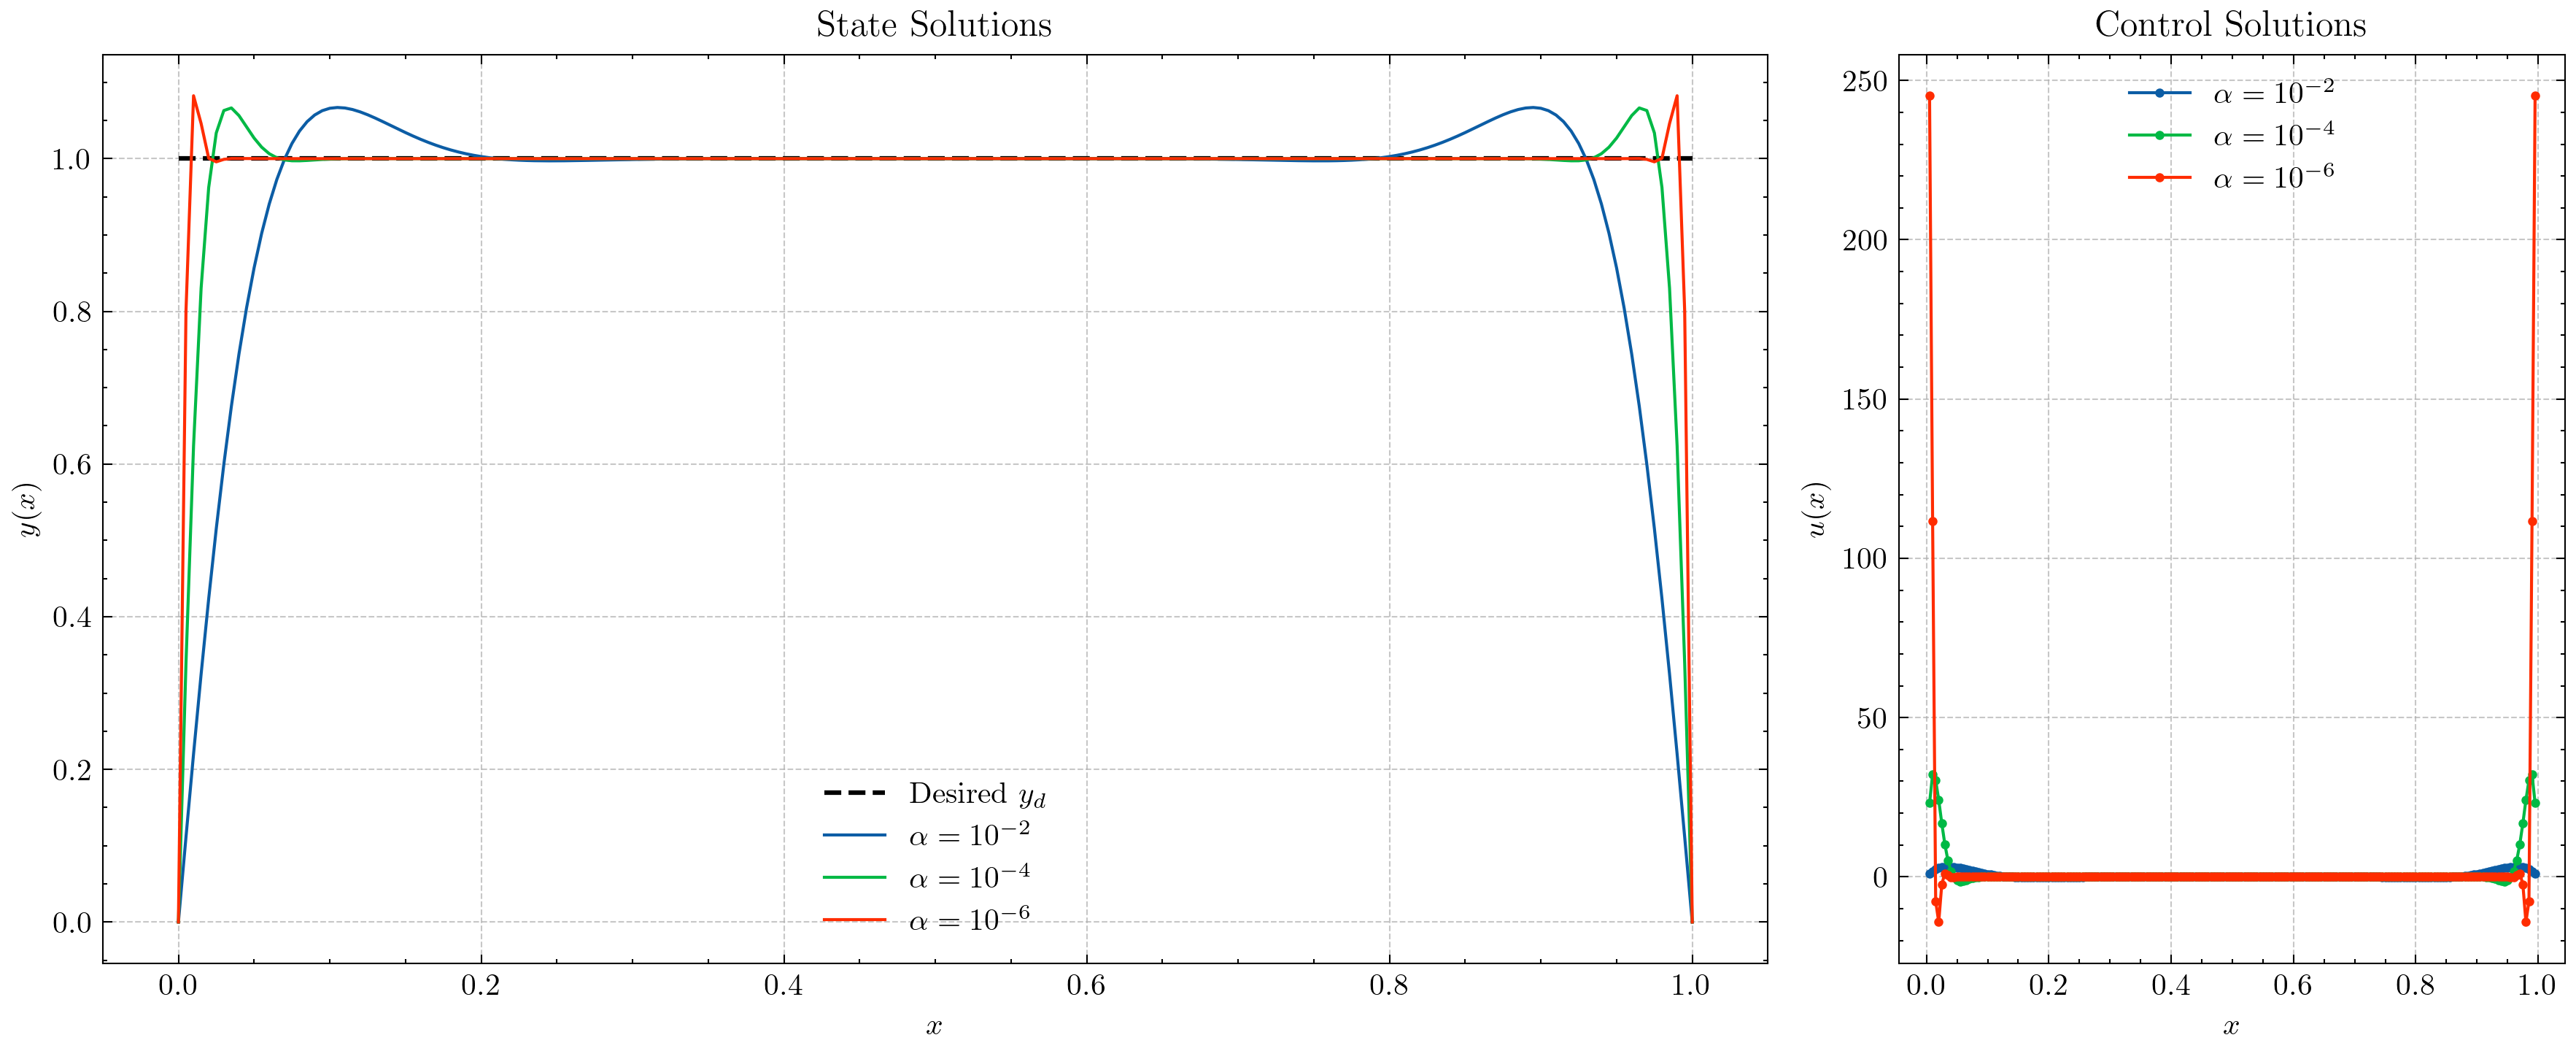
\includegraphics[width=0.95\textwidth]{figures/ocp_case2.png}
    \caption{Case~2 results: $y_h$ approaches 1 in the interior for small $\alpha$, forcing $u_h$ to grow near the boundaries.}
    \label{fig:opt_control_case2_short}
\end{figure}

\paragraph{Case 3 (discontinuous $y_d$ step function):}
For a step in $[0.25,0.75]$, large $\alpha$ again leads to $u_h\approx 0$ and $y_h\approx 0$. As $\alpha$ decreases, $y_h$ develops a plateau near 1 in the central region but must remain continuous, creating steep gradients near $x=0.25$ and $x=0.75$. Consequently, $u_h$ forms large, narrow spikes at these discontinuities.

\begin{figure}[htbp]
    \centering
    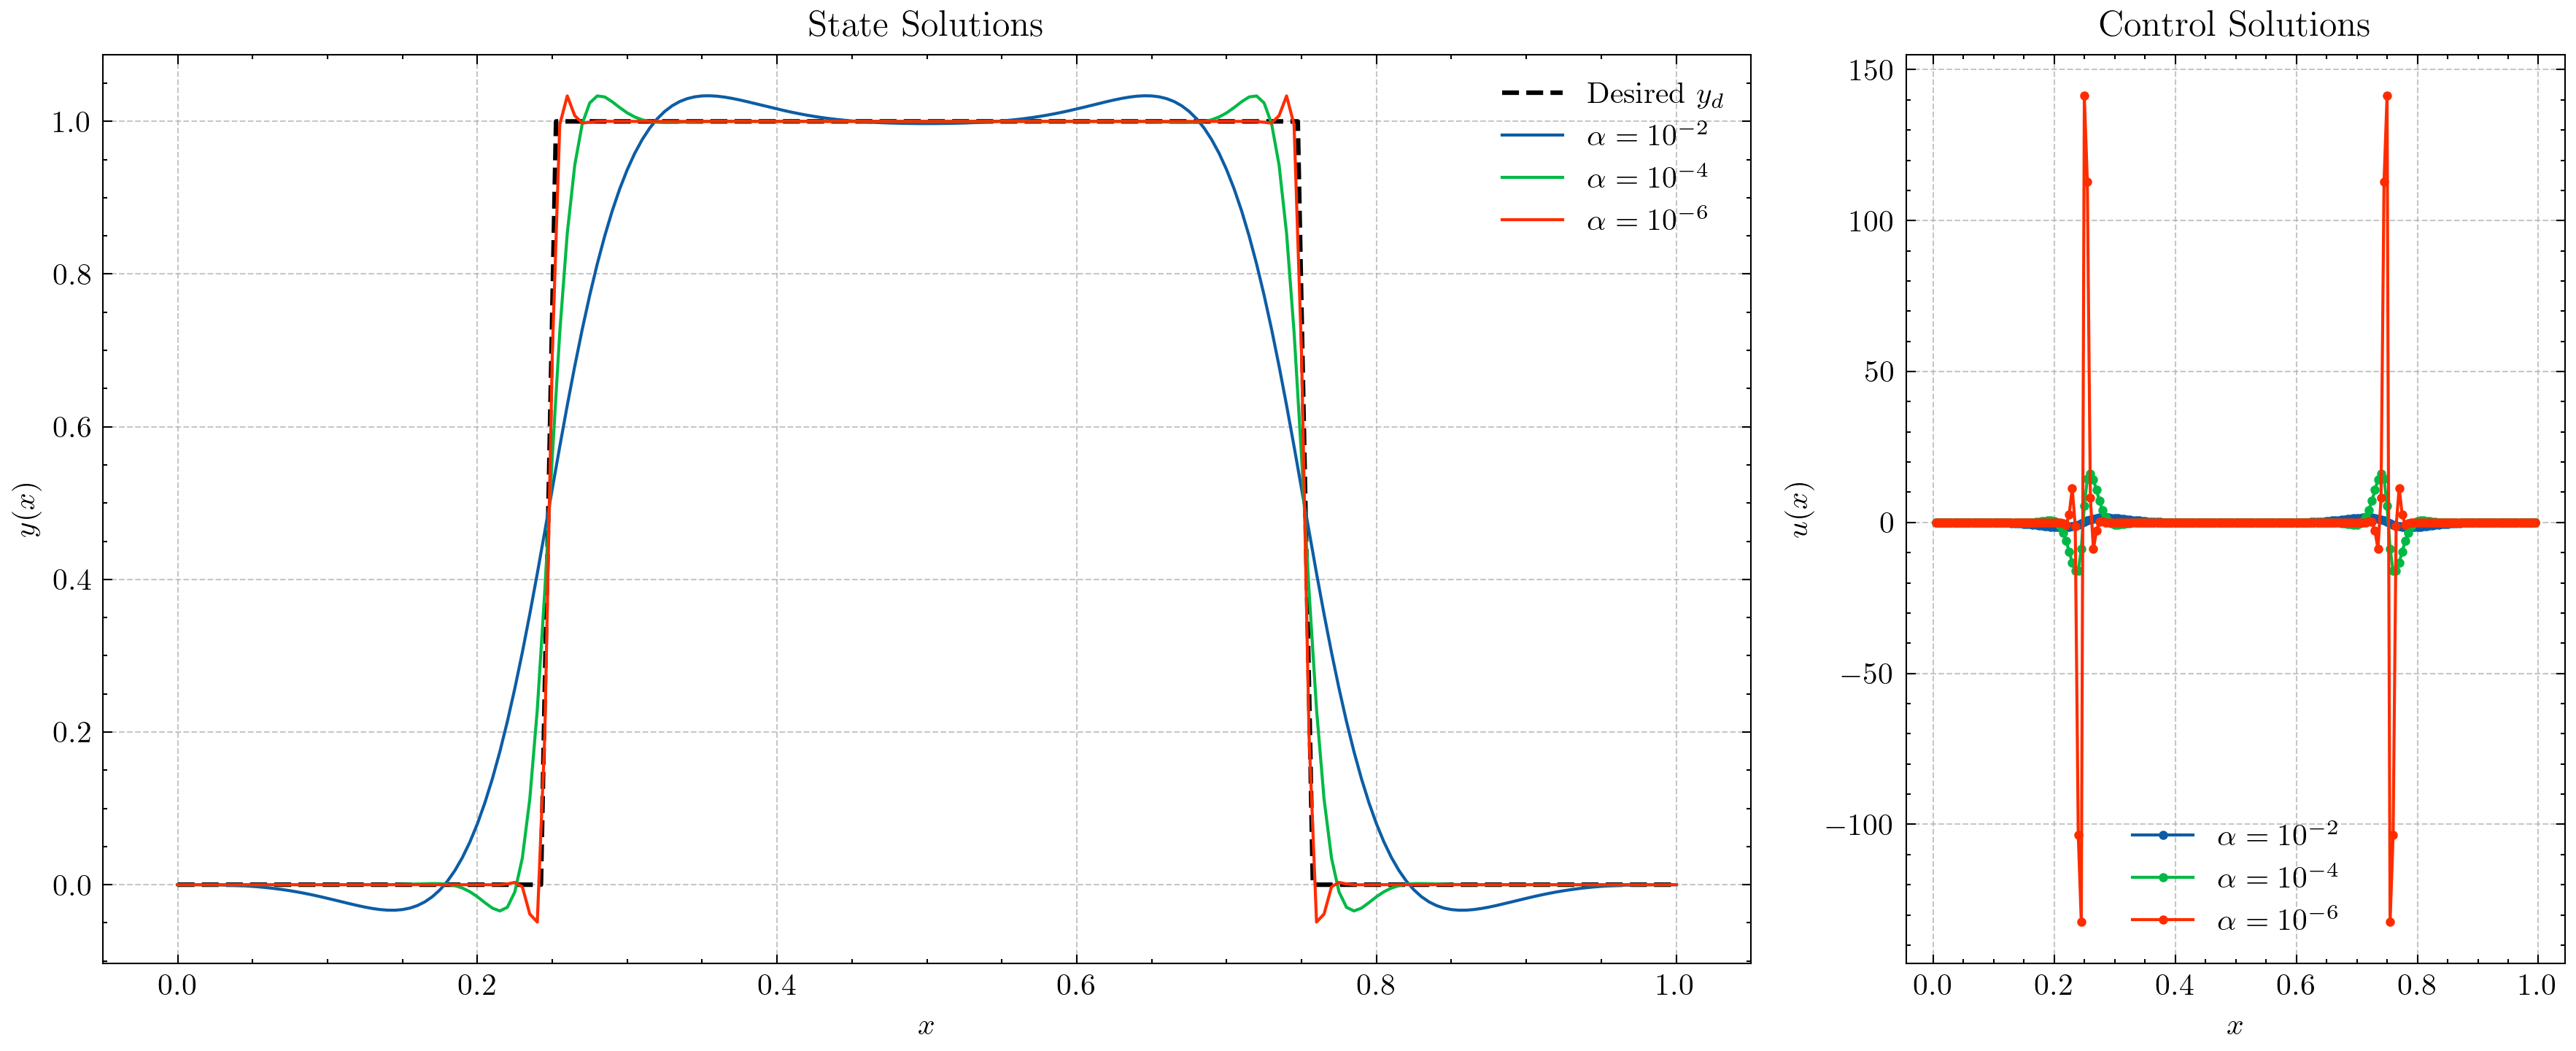
\includegraphics[width=0.95\textwidth]{figures/ocp_case3.png}
    \caption{Case~3 results: to approximate the jump, $y_h$ exhibits boundary layers and $u_h$ has localized peaks.}
    \label{fig:opt_control_case3_short}
\end{figure}

\paragraph{Effect of $\alpha$.}
Across all cases, large $\alpha$ makes control expensive, yielding $u_h\approx0$ and $y_h$ far from $y_d$. Decreasing $\alpha$ drives $y_h$ closer to $y_d$, at the cost of larger $\|u_h\|$. Intermediate values produce partial tracking with moderate control levels.

\paragraph{Regularity of $y_d$.}
When $y_d\in H^1_0(0,1)$ (Case~1), the solution can exactly attain the target for small $\alpha$. If $y_d$ is incompatible with the boundary conditions (Case~2) or is discontinuous (Case~3), then $y_h$ can only approximate $y_d$; as $\alpha\to0$, $u_h$ tends to form large spikes or boundary layers. These observations align with the theory that non-$H^1_0$ targets often induce singular (or strongly localized) optimal controls.

\subsection{Conclusion}
Our FEM-based OCP solver shows the expected interplay between the control cost $\alpha$ and the target regularity. For large $\alpha$, minimal control is used, while for small $\alpha$ the state closely matches $y_d$, potentially requiring large or sharply localized $u_h$. These results confirm that the method captures the characteristic behavior of PDE-constrained optimization for various target profiles.

\printbibliography

\end{document}